\documentclass[UTF8,10pt]{ctexart}\usepackage{graphicx, color}
%% maxwidth is the original width if it is less than linewidth
%% otherwise use linewidth (to make sure the graphics do not exceed the margin)
\makeatletter
\def\maxwidth{ %
  \ifdim\Gin@nat@width>\linewidth
    \linewidth
  \else
    \Gin@nat@width
  \fi
}
\makeatother

\IfFileExists{upquote.sty}{\usepackage{upquote}}{}
\definecolor{fgcolor}{rgb}{0.2, 0.2, 0.2}
\newcommand{\hlnumber}[1]{\textcolor[rgb]{0,0,0}{#1}}%
\newcommand{\hlfunctioncall}[1]{\textcolor[rgb]{0.501960784313725,0,0.329411764705882}{\textbf{#1}}}%
\newcommand{\hlstring}[1]{\textcolor[rgb]{0.6,0.6,1}{#1}}%
\newcommand{\hlkeyword}[1]{\textcolor[rgb]{0,0,0}{\textbf{#1}}}%
\newcommand{\hlargument}[1]{\textcolor[rgb]{0.690196078431373,0.250980392156863,0.0196078431372549}{#1}}%
\newcommand{\hlcomment}[1]{\textcolor[rgb]{0.180392156862745,0.6,0.341176470588235}{#1}}%
\newcommand{\hlroxygencomment}[1]{\textcolor[rgb]{0.43921568627451,0.47843137254902,0.701960784313725}{#1}}%
\newcommand{\hlformalargs}[1]{\textcolor[rgb]{0.690196078431373,0.250980392156863,0.0196078431372549}{#1}}%
\newcommand{\hleqformalargs}[1]{\textcolor[rgb]{0.690196078431373,0.250980392156863,0.0196078431372549}{#1}}%
\newcommand{\hlassignement}[1]{\textcolor[rgb]{0,0,0}{\textbf{#1}}}%
\newcommand{\hlpackage}[1]{\textcolor[rgb]{0.588235294117647,0.709803921568627,0.145098039215686}{#1}}%
\newcommand{\hlslot}[1]{\textit{#1}}%
\newcommand{\hlsymbol}[1]{\textcolor[rgb]{0,0,0}{#1}}%
\newcommand{\hlprompt}[1]{\textcolor[rgb]{0.2,0.2,0.2}{#1}}%

\usepackage{framed}
\makeatletter
\newenvironment{kframe}{%
 \def\at@end@of@kframe{}%
 \ifinner\ifhmode%
  \def\at@end@of@kframe{\end{minipage}}%
  \begin{minipage}{\columnwidth}%
 \fi\fi%
 \def\FrameCommand##1{\hskip\@totalleftmargin \hskip-\fboxsep
 \colorbox{shadecolor}{##1}\hskip-\fboxsep
     % There is no \\@totalrightmargin, so:
     \hskip-\linewidth \hskip-\@totalleftmargin \hskip\columnwidth}%
 \MakeFramed {\advance\hsize-\width
   \@totalleftmargin\z@ \linewidth\hsize
   \@setminipage}}%
 {\par\unskip\endMakeFramed%
 \at@end@of@kframe}
\makeatother

\definecolor{shadecolor}{rgb}{.97, .97, .97}
\definecolor{messagecolor}{rgb}{0, 0, 0}
\definecolor{warningcolor}{rgb}{1, 0, 1}
\definecolor{errorcolor}{rgb}{1, 0, 0}
\newenvironment{knitrout}{}{} % an empty environment to be redefined in TeX

\usepackage{alltt}
\usepackage[a4paper,%%textwidth=129mm,textheight=185mm,  %%193-8
text={160mm,260mm},centering]{geometry}
\pagestyle{empty}
\begin{document}
\title{用散点图示范ggplot2的核心概念}
\author{肖凯}
\maketitle
\abstract{
本文稿是第五届R语言会议演讲内容的一部分,试图用散点图示例来说明ggplot2包的核心概念,以方便初学者快速上手。同时这也是笔者应用knitr包的一个练习。该示例所用数据是ggplot2包内带的mpg数据集。}
\section{Data和Mapping}
\begin{knitrout}
\definecolor{shadecolor}{rgb}{0.969, 0.969, 0.969}\color{fgcolor}\begin{kframe}
\begin{alltt}
\hlfunctioncall{library}(ggplot2)
p <- \hlfunctioncall{ggplot}(data=mpg,mapping=\hlfunctioncall{aes}(x=cty,y=hwy))
p + \hlfunctioncall{geom_point}()
\end{alltt}
\end{kframe}

{\centering 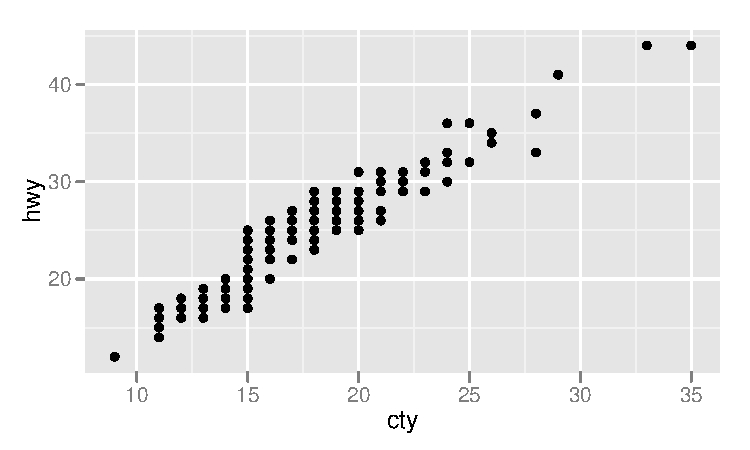
\includegraphics[width=\maxwidth]{figure/unnamed-chunk-1} 

}


\end{knitrout}

\textbf{ggplot}函数是用来构建基本的图形对象,相当于是一张空白的画布。其中我们需要定义可视化的数据对象(Data),以及数据变量到图形属性之间的映射(Mapping)。在上面的图形里, 我们使用了mpg数据框,并将cty变量映射到X轴,hwy映射到Y轴。

\section{几何对象Geom}
只有画布是不够的,还需要定义用什么样的图形来表现数据。geom代表我们能在图中实际看到的图形元素,如点、线、多边形等。在上图我们使用了point这种几何对象来展现数据,这样就画出了散点图。我们还可以用summary函数来观察图形对象的内部数据。
\begin{knitrout}
\definecolor{shadecolor}{rgb}{0.969, 0.969, 0.969}\color{fgcolor}\begin{kframe}
\begin{alltt}
\hlfunctioncall{summary}(p + \hlfunctioncall{geom_point}())
\end{alltt}
\begin{verbatim}
## data: manufacturer, model, displ, year, cyl, trans, drv, cty, hwy,
##   fl, class [234x11]
## mapping:  x = cty, y = hwy
## faceting: facet_null() 
## -----------------------------------
## geom_point: na.rm = FALSE 
## stat_identity:  
## position_identity: (width = NULL, height = NULL)
## 
\end{verbatim}
\end{kframe}
\end{knitrout}

数据不仅可以映射到数轴上,我们还可以将年份变量映射为颜色属性。
\begin{knitrout}
\definecolor{shadecolor}{rgb}{0.969, 0.969, 0.969}\color{fgcolor}\begin{kframe}
\begin{alltt}
p <- \hlfunctioncall{ggplot}(data=mpg,mapping=\hlfunctioncall{aes}(x=cty,y=hwy,colour=\hlfunctioncall{factor}(year)))
p + \hlfunctioncall{geom_point}()
\end{alltt}
\end{kframe}

{\centering 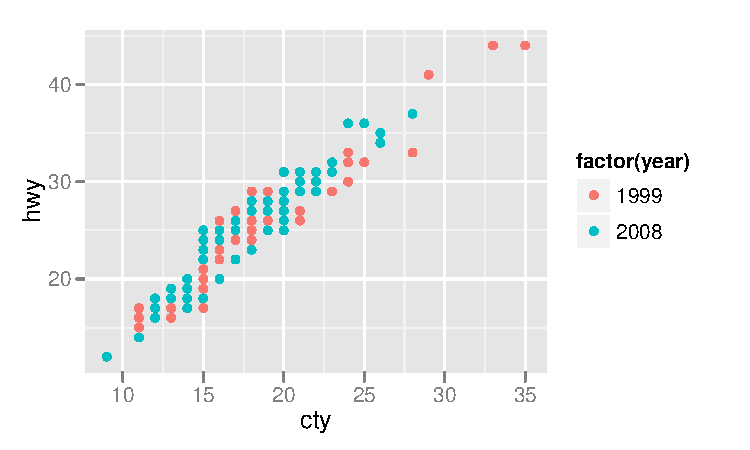
\includegraphics[width=\maxwidth]{figure/unnamed-chunk-3} 

}


\end{knitrout}

\section{统计变换Stat}
统计变换是对原始数据进行了某种提炼或归纳。散点图没有经过统计变换,它展现了数据的原貌。但有时候我们需要提炼后数据,例如下图的平滑曲线就是一种统计变换,它去除了数据的原貌。
\begin{knitrout}
\definecolor{shadecolor}{rgb}{0.969, 0.969, 0.969}\color{fgcolor}\begin{kframe}
\begin{alltt}
p <- \hlfunctioncall{ggplot}(data=mpg,mapping=\hlfunctioncall{aes}(x=cty,y=hwy,colour=\hlfunctioncall{factor}(year)))
p + \hlfunctioncall{stat_smooth}()
\end{alltt}
\end{kframe}

{\centering 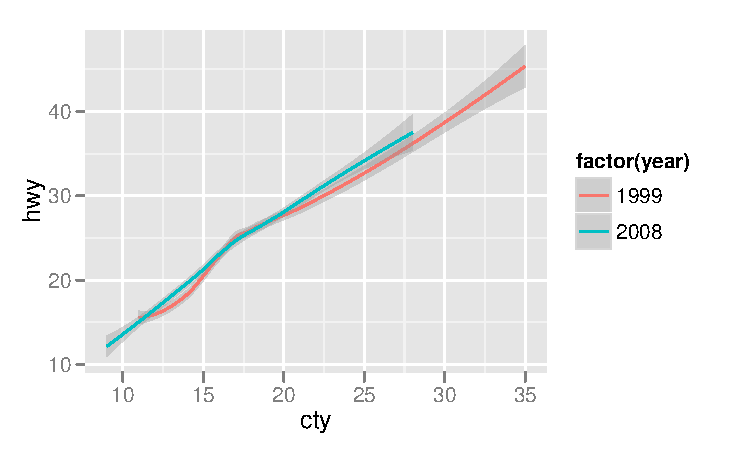
\includegraphics[width=\maxwidth]{figure/unnamed-chunk-4} 

}


\end{knitrout}

你或许会奇怪为什么会有两条平滑曲线,那是因为我们在底层画布定义了颜色属性的映射,底层的设置会影响到所有在其基础上的几何对象和统计变换。

\section{图层Layer}
我们可以将上面的散点和平滑线合并起来,如果只需要一条平滑,就需要在平滑函数中单独设置映射。
\begin{knitrout}
\definecolor{shadecolor}{rgb}{0.969, 0.969, 0.969}\color{fgcolor}\begin{kframe}
\begin{alltt}
p <- \hlfunctioncall{ggplot}(data=mpg,mapping=\hlfunctioncall{aes}(x=cty,y=hwy))
p + \hlfunctioncall{geom_point}(\hlfunctioncall{aes}(colour=\hlfunctioncall{factor}(year)))  + \hlfunctioncall{stat_smooth}()
\end{alltt}
\end{kframe}

{\centering 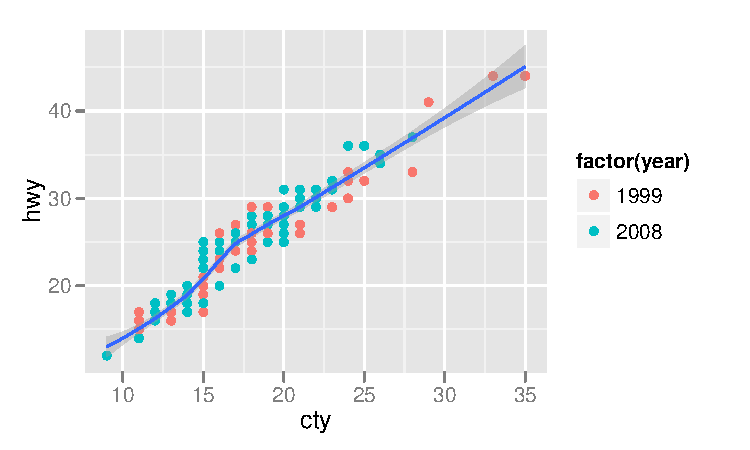
\includegraphics[width=\maxwidth]{figure/unnamed-chunk-5} 

}


\end{knitrout}

下面的命令和之前的是等价的。
\begin{knitrout}
\definecolor{shadecolor}{rgb}{0.969, 0.969, 0.969}\color{fgcolor}\begin{kframe}
\begin{alltt}
p <- \hlfunctioncall{ggplot}()
d <- p + \hlfunctioncall{geom_point}(data=mpg, mapping=\hlfunctioncall{aes}(x=cty,y=hwy,colour=\hlfunctioncall{factor}(year))) + 
         \hlfunctioncall{stat_smooth}(data=mpg, mapping=\hlfunctioncall{aes}(x=cty,y=hwy))
\hlfunctioncall{print}(d)
\end{alltt}
\end{kframe}
\end{knitrout}

这时我们可以引入图层的概念了,一个图层好比是一张玻璃纸,包含有各种图形元素,你可以分别建立图层然后叠放在一起,组合成图形的最终效果。图层可以允许用户一步步的构建图形,方便单独对图层进行修改、增加统计量、甚至改动数据。

如果我们观察d对象中的信息,会发现一些有趣的东西。这里除了底层画布之外,有两个图层,分别是几何对象散点和统计变换平滑线。仔细观察会发现几何对象层中有一个默认为空的统计变换stat,而统计变换层中也有一个默认的geom,毕竟提炼后的数据也需要一种几何图形来展现。
\begin{knitrout}
\definecolor{shadecolor}{rgb}{0.969, 0.969, 0.969}\color{fgcolor}\begin{kframe}
\begin{alltt}
\hlfunctioncall{summary}(d)
\end{alltt}
\begin{verbatim}
## data: [x]
## faceting: facet_null() 
## -----------------------------------
## mapping: x = cty, y = hwy, colour = factor(year) 
## geom_point: na.rm = FALSE 
## stat_identity:  
## position_identity: (width = NULL, height = NULL)
## 
## mapping: x = cty, y = hwy 
## geom_smooth:  
## stat_smooth: method = auto, formula = y ~ x, se = TRUE, n = 80, fullrange = FALSE, level = 0.95, na.rm = FALSE 
## position_identity: (width = NULL, height = NULL)
## 
\end{verbatim}
\end{kframe}
\end{knitrout}

\section{标度Scale}
映射只负责将变量关联到某个图形属性,但并不负责具体的取值。例如Mapping参数将年份变量映射到颜色属性,但具体哪一年用哪种颜色显示,它并不管。谁来管呢?由标度来控制。通常用户可以不用去关注标度,ggplot2系统会自动处理细节,但当用户想干预的时候,就可以出手。如果我们不满意之前的颜色,可以用下面的标度函数设置需要的色彩。
\begin{knitrout}
\definecolor{shadecolor}{rgb}{0.969, 0.969, 0.969}\color{fgcolor}\begin{kframe}
\begin{alltt}
p <- \hlfunctioncall{ggplot}(data=mpg,mapping=\hlfunctioncall{aes}(x=cty,y=hwy))
p + \hlfunctioncall{geom_point}(\hlfunctioncall{aes}(colour=\hlfunctioncall{factor}(year)))+
    \hlfunctioncall{scale_color_manual}(values =\hlfunctioncall{c}(\hlstring{'blue2'},\hlstring{'red4'}))+
    \hlfunctioncall{stat_smooth}()
\end{alltt}
\end{kframe}

{\centering 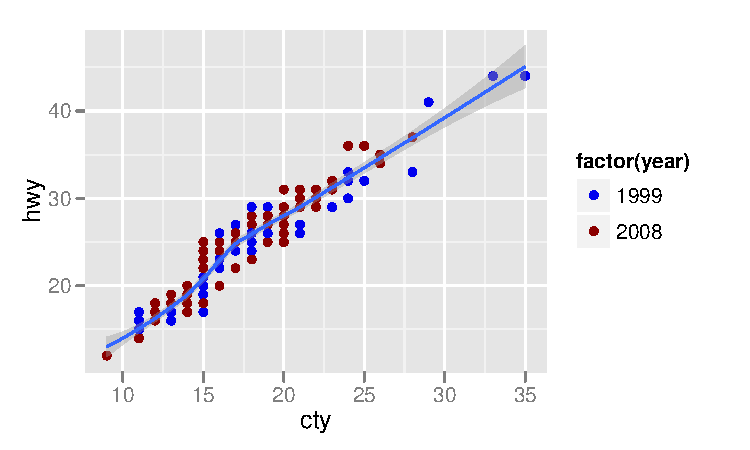
\includegraphics[width=\maxwidth]{figure/unnamed-chunk-8} 

}


\end{knitrout}

\section{分面Facet}
条件绘图是将数据按某种方式分组后分别绘图。分面就是控制条件绘图的方法和排列形式。下图就是将数据按年份变量分组后绘图。这只需要增加一行简单的代码,从中可以看到ggplot的威力在于可以逐步的修改、完善图形。
\begin{knitrout}
\definecolor{shadecolor}{rgb}{0.969, 0.969, 0.969}\color{fgcolor}\begin{kframe}
\begin{alltt}
p <- \hlfunctioncall{ggplot}(data=mpg,mapping=\hlfunctioncall{aes}(x=cty,y=hwy))
p + \hlfunctioncall{geom_point}(\hlfunctioncall{aes}(colour=\hlfunctioncall{factor}(year)))+
    \hlfunctioncall{scale_color_manual}(values =\hlfunctioncall{c}(\hlstring{'blue2'},\hlstring{'red4'}))+
    \hlfunctioncall{stat_smooth}()+
    \hlfunctioncall{facet_wrap}(~ year,ncol=1)
\end{alltt}
\end{kframe}

{\centering 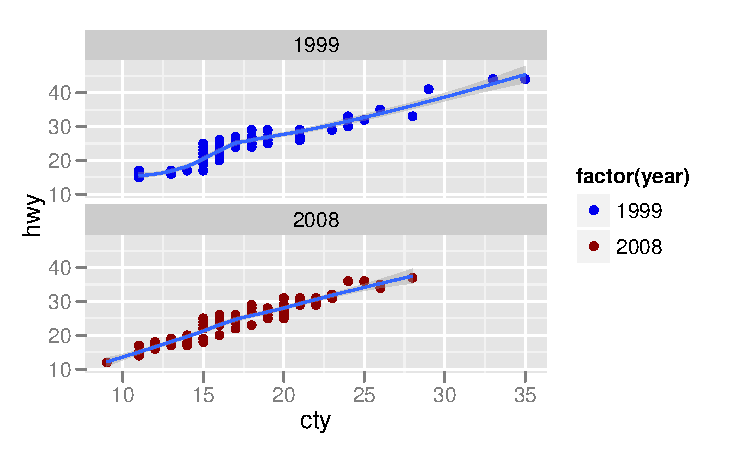
\includegraphics[width=\maxwidth]{figure/unnamed-chunk-9} 

}


\end{knitrout}

\section{最后的调整}
下面我们要对图形精细调整,首先用透明度和扰动解决上图中点的重叠问题,此外还要将排量映射为点的大小。最后增加图名和图例名称。
\begin{knitrout}
\definecolor{shadecolor}{rgb}{0.969, 0.969, 0.969}\color{fgcolor}\begin{kframe}
\begin{alltt}
p <- \hlfunctioncall{ggplot}(data=mpg,mapping=\hlfunctioncall{aes}(x=cty,y=hwy))
p + \hlfunctioncall{geom_point}(\hlfunctioncall{aes}(colour=class,size=displ), alpha=0.5,position = \hlstring{"jitter"})+
    \hlfunctioncall{stat_smooth}()+
    \hlfunctioncall{facet_wrap}(~ year,ncol=1)+
    \hlfunctioncall{opts}(title=\hlstring{'fuel economy of car'})+
    \hlfunctioncall{labs}(y=\hlstring{'highway miles per gallon'},
         x=\hlstring{'city miles per gallon'})
\end{alltt}
\end{kframe}

{\centering 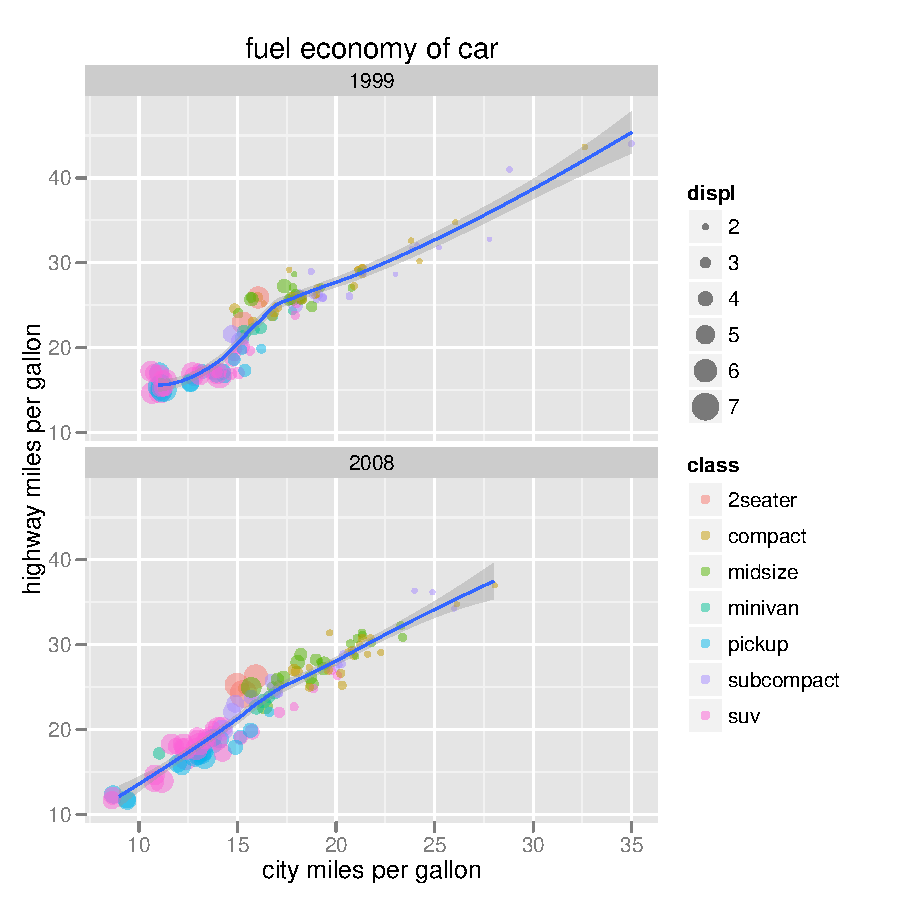
\includegraphics[width=\maxwidth]{figure/unnamed-chunk-10} 

}


\end{knitrout}


ggplot2中几个重要的核心概念都已经涉及到了,还有坐标系统和位置调整没有提到。希望这篇短文对你有用,由此进入ggplot2的世界,领略数据可视化的力与美。各位也可访问我的博客作进一步的交流。xccds1977.blogspot.com(需翻墙),或是给我发电邮xccds1977@gmail.com。
\end{document}
